\section{Свойства степенных рядов}\label{sec-power-series-03}

\begin{theorem}[Сходимость внутри круга]\label{thm-power-uniform}

Пусть \(R>0\) --- радиус ряда \eqref{eq-power-series}. Для каждого \(0<r<R\) ряд сходится равномерно на \(|z-z_0|\le r\) и абсолютно в каждой точке \(|z-z_0|<R\).

\end{theorem}

\begin{proof}

По определению \(R\) существует точка сходимости, расстояние которой от центра больше \(r\). Применяем теорему \ref{thm-abel-first}.

\end{proof}

\begin{theorem}[Непрерывность суммы]\label{thm-power-continuity}

Сумма \(S(z)=\sum_{n=0}^\infty c_n(z-z_0)^n\) непрерывна внутри круга \(|z-z_0|<R\).

\end{theorem}

\begin{proof}

Для любой точки \(z^*\) внутри круга выбираем \(r\) с \(|z^*-z_0|<r<R\). На \(|z-z_0|\le r\) ряд сходится равномерно, а каждый его член непрерывен. По теореме \ref{thm-series-continuity} сумма непрерывна в \(z^*\).

\end{proof}

\begin{center}
\begin{minipage}{\linewidth}
\centering
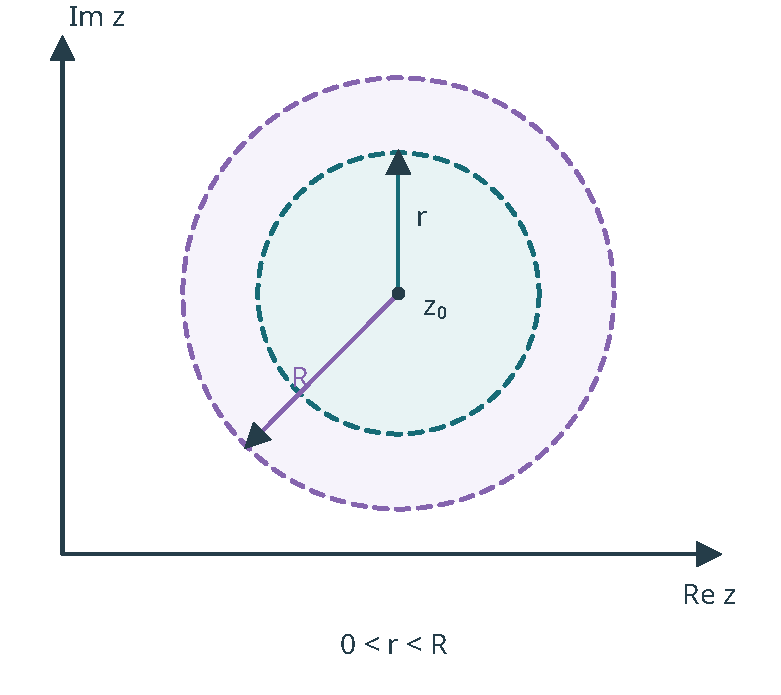
\includegraphics[width=0.65\linewidth]{figures/disks.pdf}
\captionof{figure}{Круг сходимости радиуса R и вложенный круг радиуса r с равномерной сходимостью.}\label{fig-disks}
\end{minipage}
\end{center}

\begin{cor}[Вторая теорема Абеля: радиальный предел]\label{cor-abel-second}

Пусть \(0<R<+\infty\) и ряд сходится в граничной точке \(z^*\), \(|z^*-z_0|=R\). Тогда

\begin{equation}
\lim_{t\to1-}S\bigl(z_0+t(z^*-z_0)\bigr)=S(z^*),
\qquad 0\le t<1.
\label{eq-abel-radial}
\end{equation}

В вещественном случае это непрерывность суммы при подходе к концу интервала изнутри.

\end{cor}

При условной сходимости на границе гарантируется радиальный предел. Если \(\sum|c_n|R^n<\infty\), то по Вейерштрассу ряд равномерно сходится на замкнутом круге и сумма непрерывна на всей его границе.

\begin{proof}

Обозначим \(b_n=c_n(z^*-z_0)^n\). Числовой ряд \(\sum b_n\) сходится. Рассматриваем его как функциональный ряд постоянных функций на \([0,1]\): он сходится равномерно. Множители \(v_n(t)=t^n\) монотонны по \(n\) при каждом \(t\in[0,1]\) и ограничены единицей. По теореме \ref{thm-abel-test} ряд \(\sum b_nt^n\) сходится равномерно на \([0,1]\). Его сумма непрерывна, что даёт формулу \eqref{eq-abel-radial}.

\end{proof}

\subsection{Дифференцирование}\label{sec-power-series-03-1}

\begin{theorem}[Производная суммы степенного ряда]\label{thm-power-derivative}

Внутри круга сходимости

\begin{equation}
S'(z)=\sum_{n=1}^\infty nc_n(z-z_0)^{n-1}.
\label{eq-power-derivative}
\end{equation}

Радиус производного ряда равен \(R\), а \(S'\) непрерывна внутри круга.

\end{theorem}

\begin{proof}

Сдвигом полагаем \(z_0=0\). Сначала ряд \(\sum_{n=1}^\infty nc_nz^n\) имеет тот же радиус, поскольку \(n^{1/n}\to1\): \[
\limsup_n\sqrt[n]{n|c_n|}=\limsup_n\sqrt[n]{|c_n|}=1/R.
\] Сдвиг показателя степени на единицу также сохраняет радиус: при \(z\ne0\) ряд \(\sum nc_nz^{n-1}\) --- это \(z^{-1}\sum nc_nz^n\); в нуле оба ряда определены. Поэтому производный ряд имеет радиус \(R\).

Фиксируем \(z^*\) с \(|z^*|<R\) и выбираем \(r\) с \(|z^*|<r<R\). Для \(z\ne z^*\), \[
\frac{S(z)-S(z^*)}{z-z^*}
=\sum_{n=1}^\infty c_n\frac{z^n-(z^*)^n}{z-z^*}.
\] Каждый член справа продолжается в \(z=z^*\) как полином \[
u_n(z)=c_n\bigl(z^{n-1}+z^{n-2}z^*+\cdots+(z^*)^{n-1}\bigr).
\] При \(|z|\le r\), \(|z^*|<r\) получаем \(|u_n(z)|\le|c_n|nr^{n-1}\). Числовой ряд этих мажорант сходится, поскольку \(r<R\). По теореме \ref{thm-weierstrass} ряд \(\sum u_n(z)\) сходится равномерно и имеет непрерывную сумму. Поэтому \[
\lim_{z\to z^*}\frac{S(z)-S(z^*)}{z-z^*}
=\sum_{n=1}^\infty\lim_{z\to z^*}u_n(z)
=\sum_{n=1}^\infty nc_n(z^*)^{n-1}.
\] Непрерывность \(S'\) следует из теоремы \ref{thm-power-continuity} для производного ряда.

\end{proof}

\begin{cor}[Производные всех порядков]\label{cor-power-higher-derivatives}

Сумма степенного ряда бесконечно дифференцируема внутри круга сходимости, и для каждого \(k\ge0\)

\begin{equation}
S^{(k)}(z)=\sum_{n=k}^\infty c_n\frac{n!}{(n-k)!}(z-z_0)^{n-k}.
\label{eq-power-higher-derivatives}
\end{equation}

Все эти производные непрерывны внутри круга.

\end{cor}

Доказательство --- последовательное применение теоремы \ref{thm-power-derivative}.

\subsection{Интегрирование}\label{sec-power-series-03-2}

\begin{theorem}[Почленное интегрирование вещественного ряда]\label{thm-power-integral}

Пусть \(S(x)=\sum_{n=0}^\infty c_n(x-x_0)^n\), где \(c_n,x_0\in\mathbb R\), \(R>0\). Если \([a,b]\subset(x_0-R,x_0+R)\), то \(S\in R([a,b])\) и

\begin{equation}
\begin{aligned}
\int_a^b S(x)\,dx
&=\sum_{n=0}^\infty c_n\int_a^b \bigl((x-x_0)^n\bigr)\,dx\\
&=\sum_{n=0}^\infty\frac{c_n}{n+1}
\left((b-x_0)^{n+1}-(a-x_0)^{n+1}\right).
\end{aligned}
\label{eq-power-integral}
\end{equation}

\end{theorem}

\begin{proof}

Отрезок \([a,b]\) содержится в меньшем отрезке \(|x-x_0|\le r<R\). Ряд на нём сходится равномерно. Применяем теорему \ref{thm-series-integral}.

\end{proof}
